\documentclass[11pt,a4paper]{amsart}
\usepackage[utf8]{inputenc}
\usepackage{amsmath}
\usepackage{amsfonts}
\usepackage{amssymb}
\usepackage{graphicx}
\usepackage{mathtools}
\usepackage{amsthm,amssymb}
\usepackage[margin=1in]{geometry}
\usepackage[T1]{fontenc}

%------------------------------------------------------------
% Theorem like environments
%
\newtheorem{theorem}{Theorem}
\theoremstyle{plain}
\newtheorem{acknowledgement}{Acknowledgement}
\newtheorem{algorithm}{Algorithm}
\newtheorem{axiom}{Axiom}
\newtheorem{case}{Case}
\newtheorem{claim}{Claim}
\newtheorem{conclusion}{Conclusion}
\newtheorem{condition}{Condition}
\newtheorem{conjecture}{Conjecture}
\newtheorem{corollary}{Corollary}
\newtheorem{criterion}{Criterion}
\newtheorem{definition}{Definition}
\newtheorem{example}{Example}
\newtheorem{exercise}{Exercise}
\newtheorem{lemma}{Lemma}
\newtheorem{notation}{Notation}
\newtheorem{problem}{Problem}
\newtheorem{proposition}{Proposition}
\newtheorem{remark}{Remark}
\newtheorem{solution}{Solution}
\newtheorem{summary}{Summary}
\numberwithin{equation}{section}
%--------------------------------------------------------

\begin{document}
\title{BINARY HEAP}
\author{NITHIN JOSHUA STEPHEN - CS14M033}
%\address{M.Tech 1^(st) year, CSE Department, IIT Madras}
%\email{nithinjs.88@gmail.com}
\date{25-Aug-2014}

\begin{abstract}
\noindent
\centering
This document gives a brief overview of binary heap data structure \\ and operations associated with it.
\end{abstract}
\maketitle

\section{\textbf{Introduction}}

A \textbf{binary heap} is a data structure similar to binary tree with two additional constraints.

	1) \textbf{Heap Property}: The value of children of an element must be always less than \textbf{(max-heap)} or always greater than \textbf{(min-heap)} the value of it's parent. However, there is no constraint for values between the siblings of an element.
	
	2) \textbf{Shape property}: The binary heap is a \emph{complete} tree where all levels, except the lowest level with height $0$ is completely filled.
	
\begin{figure}[h] \label{fig:minheap}
\centering
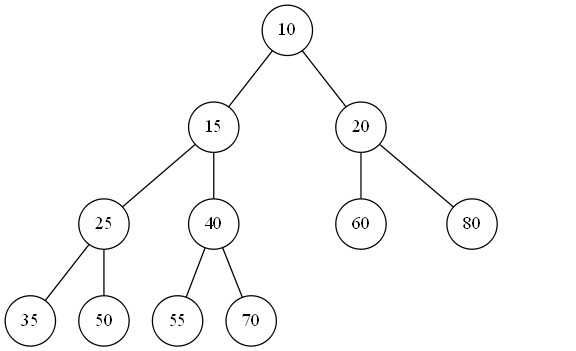
\includegraphics[scale=0.4]{minheap}
\caption{min-heap}
\end{figure}

\section{\textbf{Operations}}
A binary minheap has the following operations associated with it
\begin{itemize}
	\item \textbf{MIN-HEAPIFY}: It maintains the \textit{Heap property} where an element's left and right subtrees are valid min-heaps, but the subtree rooted at it is not a min-heap.
	\item \textbf{INSERT}: It inserts the element into a min-heap.
	\item \textbf{EXTRACT-MIN}: It removes the element and returns it.
\end{itemize}
\section{\textbf{Implementation}}

A binary heap is an \emph{Abstract Data Type} implemented either using an array or pointers similar to binary tree. 
\subsection{Using array}
	If min-heap is implemented using an array, attributes associated with are
	\begin{itemize}
		\item \texttt{size}: It indicates the number of elements in a min-heap.
		\\The root is \texttt{array[0]} and the last element is \texttt{array[size-1]}
	\end{itemize}
	The auxillary operations associated with it are
	\begin{itemize}
		\item The \emph{parent} of an element of index $i$ is given by
		$\displaystyle{\left\lceil{\displaystyle{\frac{i}{2}}}\right\rceil}-1$
		\item The \emph{left child} of an element of index $i$ is given $2*i + 1$
		\item The \emph{right child} of an element of index $i$ is given $2*(i + 1)$
	\end{itemize}
\subsection{Using pointers}
\noindent If implemented using pointers, attributes associated with are
\begin{enumerate}
	\item \texttt{root}: It points to the root of the min-heap.
	\item \texttt{tail}: It points to the last element of the min-heap.
	\item \texttt{parent}: This is associated with each element and it points to the parent of the element.
	\item \texttt{left child}: This is associated with each element and it points to the left child of the element.
	\item \texttt{right child}: This is associated with each element and it points to the right child of the element.
\end{enumerate}

\section{\textbf{Height of a heap}}
The height of an element in heap is the number of edges on the longest downward path from the element to a leaf and the height of the heap is the height of the root. The height $h$ of the heap is \textbf{$O(log_2n)$} where $n$ is the number of elements in a heap. The worst case for height $h$ occurs when there is \emph{only 1 element in last level}

\indent No of elements in level $0 = 2^0 = 1$\\
\indent No of elements in level $1 = 2^1 = 2$\\
\indent No of elements in level $2 = 2^2 = 4$\\
\indent No of elements in level $i = 2^i$\\
\indent No of elements in last but one level $i = 2^{h-1}$\\
\indent No of elements in last level $= 1$\\
Adding all the elements at each level\\
\indent $\sum\limits_{i=0}^h = 1 + 2 + 4 .. 2^{h-1} + 1 = 2^h$\\
So number of elements $n$ = $2^h$
$\implies$ $h$ = $log_2n$ $\implies h=O(log_2n)$ 


\section{\textbf{Working of INSERT operation}}

The INSERT operation add the element at the last index, which may cause violation of \textit{Heap property}. The inserted element is compared with its parent. If the parent is greater than the element, they are swapped to maintain \textit{Heap property}. Then the parent is compared with its parent and the swaps continue up the heap until an element is greater than its parent.\\
\indent Consider inserting 18. The following operations happen during insertion.

\indent1) element 18 is compared with element 60 and they are swapped as 18 < 60\\
\indent2) element 18 is compared with element 20 and they are swapped as 18 < 20\\
\indent3) element 18 is compared with element 10 and insert operation terminates as 18 > 10

\begin{figure}[h] \label{fig:png}
\centering
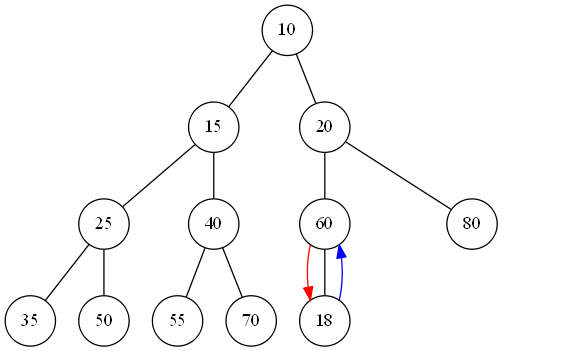
\includegraphics[scale=0.3]{insert1}
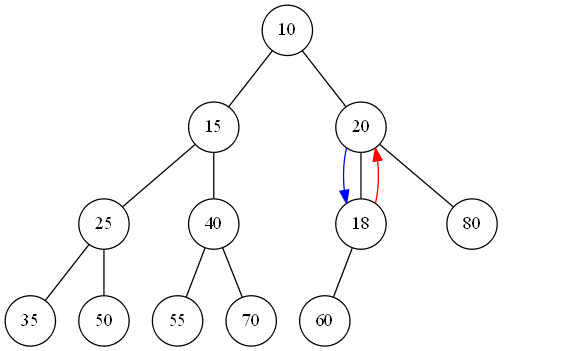
\includegraphics[scale=0.3]{insert2}
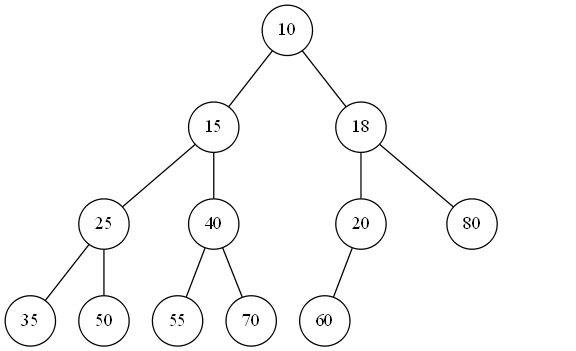
\includegraphics[scale=0.3]{insert3}
\caption{Inserting 18 into min-heap}
\end{figure}

\paragraph{}
\noindent The INSERT operation happens up the heap and the worst case number of swaps occur when the element inserted is less than the root, where swaps happen all the way up to the root. So maximum number of swaps is equal to height of the heap and hence running time is $O(h)$ or $O(log_2n)$ 

\section{\textbf{Working of EXTRACT-MIN operation}}
	EXTRACT-MIN operation removes and returns the minimum element in a min-heap. The minimum element is at the root of the heap. It is swapped with the tail and removed from the heap. The new root is compared with it's children. If it is less,  the process is stopped, else the root is swapped with the smallest of the children and this process continues down the heap until the parent element is smaller than it's children.  When the swapping process finishes the removed element is returned.

\indent The following operations happen during EXTRACT-MIN operation.

\indent 1) element 70 is swapped with element 10(ie root) and removed\\
\indent 2) element 70 is compared with element 15 and they are swapped as 70 > 15\\
\indent 3) element 70 is compared with element 25 and they are swapped as 70 > 25\\
\indent 4) element 70 is compared with element 35 and they are swapped as 70 > 35\\
\indent 5) element 70 is now a leaf, and element 10 is returned

\begin{figure}[h] \label{fig:png}
\centering
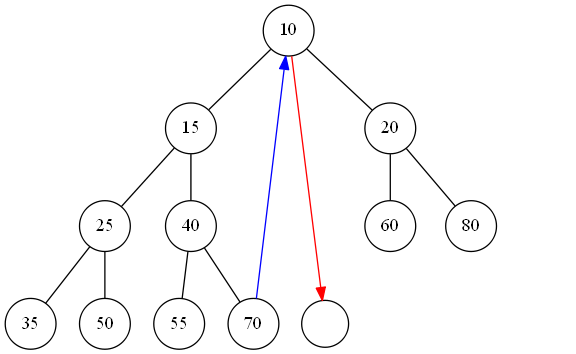
\includegraphics[scale=0.3]{delete1}
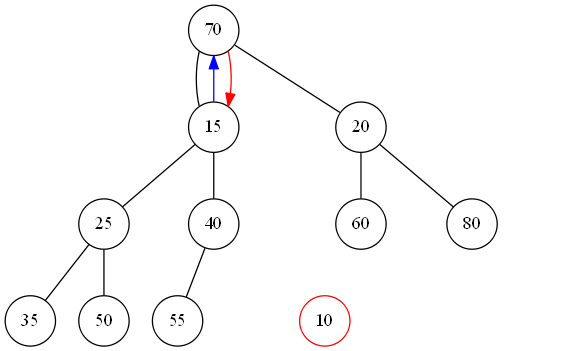
\includegraphics[scale=0.3]{delete2}
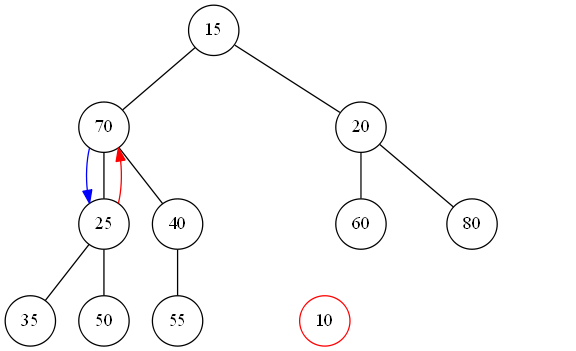
\includegraphics[scale=0.3]{delete3}
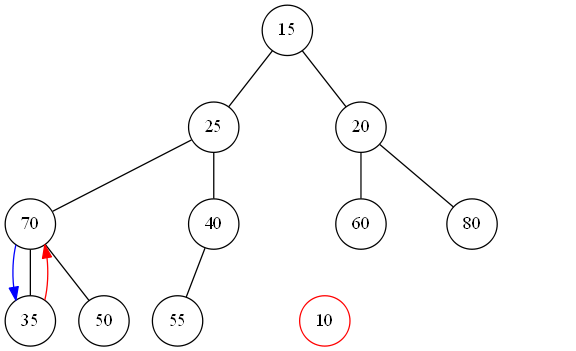
\includegraphics[scale=0.3]{delete4}
\caption{extract-min operation}
\end{figure}

\paragraph{}
\noindent The EXTRACT-MIN operation happens down the heap and the worst case number of swaps occur when the swaps happen all the way up to a leaf. So maximum number of swaps is equal to height of the heap and hence running time is $O(h)$ or $O(log_2n)$
\\
\begin{thebibliography}{}
\bibitem {}Thomas H. Cormen ,Charles E. Leiserson ,Ronald L. Rivest,Clifford Stein, \textit{Introduction to Algorithms, 2nd edition}, 2006
\bibitem{} web resource \textit{wikipedia}
\end{thebibliography}
\end{document}
\end{document}